\documentclass[MASTER.tex]{subfiles}
\begin{document}
	%====================================================%
	\begin{frame}
		\frametitle{pandas}
		\large
		\begin{figure}
			\centering
			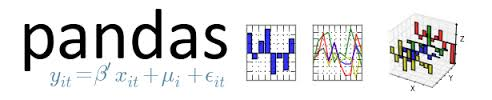
\includegraphics[width=0.7\linewidth]{pandaslogo}
		\end{figure}
		\begin{itemize}
			\item pandas is a high-performance module that provides a comprehensive set of structures for working with
			data. 
			\item pandas excels at handling structured data, such as data sets containing many variables, working with
			missing values and merging across multiple data sets. 
		\end{itemize}
	\end{frame}
%==============================================%
\begin{frame}
\begin{figure}
\centering
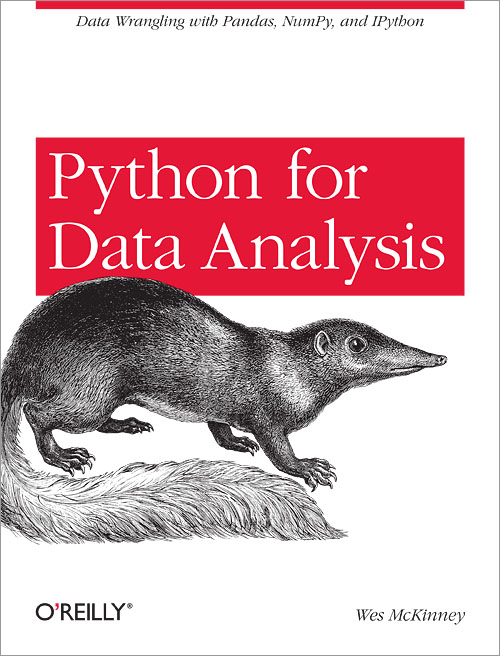
\includegraphics[width=0.75\linewidth]{pydatabook}

\end{figure}


\end{frame}

%====================================================%
\begin{frame}
	\frametitle{pandas}
	\large


	\begin{itemize}
	\item While extremely useful, pandas is not an essential
	component of the Python scientific stack unlike NumPy, SciPy or matplotlib, and so while pandas doesn’t
	make data analysis possible in Python, it makes it much easier. \item pandas also provides high-performance,
	robust methods for importing from and exporting to a wide range of formats.
	\end{itemize}
\end{frame}
%====================================================%
\begin{frame}
	\frametitle{pandas}
\textbf{Data Structures}\\
pandas provides a set of data structures which include Series, DataFrames and Panels.
\begin{itemize}
\item \textbf{Series} are 1-dimensional
	arrays.
	\item \textbf{DataFrames} are collections of Series and so are 2-dimensional, 
\item  \textbf{Panels} are collections ofDataFrames,
	and so are 3-dimensional.
	\end{itemize}
\end{frame}

\end{document}
